\documentclass[landscape,a0paper,fontscale=0.292]{baposter}

\usepackage[vlined]{algorithm2e}
\usepackage{times}
\usepackage{calc}
\usepackage{url}
\usepackage{graphicx}
\usepackage{amsmath}
\usepackage{amssymb}
\usepackage{multirow}
\usepackage{booktabs}
\usepackage{array}

\usepackage{graphicx}
\usepackage{multicol}
\usepackage[T1]{fontenc}
\usepackage{ae}

\usepackage{colortbl}
\usepackage{xcolor}
\graphicspath{{images/}}

\setlength{\columnsep}{0.7em}
\setlength{\columnseprule}{0mm}

\newcommand{\compresslist}{%
\setlength{\itemsep}{0pt}%
\setlength{\parskip}{0pt}%
\setlength{\parsep}{0pt}%
}
\renewcommand{\rmdefault}{ptm} % Times
\renewcommand{\sfdefault}{ptm} % Times

\begin{document}
\begin{poster}{
 grid=false,
 columns=5,
 colspacing=0.7em,
 headerColorOne=cyan!20!white!90!black,
 borderColor=cyan!30!white!90!black,
 textborder=faded,
 headerborder=open,
 headershape=roundedright,
 headershade=plain,
 background=none,
 bgColorOne=cyan!10!white,
 headerheight=0.12\textheight}
 % Eye Catcher
 {
  
\includegraphics[width=0.14\linewidth]{./hkust_logo_horizontal_1267x399}
 }
 % Title
{\sc\huge\bf RotateAttention: RoPE-Aware Rotation and\\ Range Rectification for INT4 Quantized\\ Attention in Video Generation}
 % Authors
 {\vspace{0.3em} Yaofu Liu, Wanli Lan, Jinxi Li, Binhang Yuan, Harry Yang}
 % University logo / tagline
 {
  
\includegraphics[width=0.18\linewidth]{logo}
 }

%%%%%%%%%%%%%%%%%%%%%%%%%%%%%%%%%%%%%%%%%%%%%%%%%%%%%%%%%%%%%%%%%%%%%%%%%%%%%%
\headerbox{\bf\color{blue} Problem Definition \& Contribution}{name=problem,column=0,row=0,span=2}{
    \textbf{\color{blue}Goal:} Fast, accurate \textbf{INT4 quantized FlashAttention} for \textbf{3D-RoPE video DiTs} (sequences $>10$K tokens, quadratic cost).
    \begin{itemize}\compresslist
        \item \textbf{C1:} online rotation (the usual Q/K outlier remedy) is hard to reconcile with \textbf{3D RoPE}.
        \item \textbf{C2:} $\mathbf{P}\in(0,1]$ makes symmetric INT4 waste \emph{half} of the range.
        \item \textbf{Observation:} 3D RoPE induces structured, \emph{segmental} Q/K outliers with cross-matrix symmetry.
    \end{itemize}

    \textbf{\color{blue}Contributions:}
    \begin{itemize}\compresslist
        \item \textbf{RoPE-aware Rotation} (Interleaved/Half) equalizes 3D-RoPE outliers at zero/negligible cost.
        \item \textbf{Key finding: rotation matrices must be orthogonal}; unconstrained rotations amplify quantization error.
        \item \textbf{Range-optimized $\mathbf{P}$} and \textbf{Hadamard $\mathbf{V}$} (zero cost) complete the INT4 pipeline.
        \item Up to \textbf{2.2$\times$} kernel / \textbf{1.68$\times$} end-to-end speedup, near-FP16 quality.
    \end{itemize}

    \begin{center}
        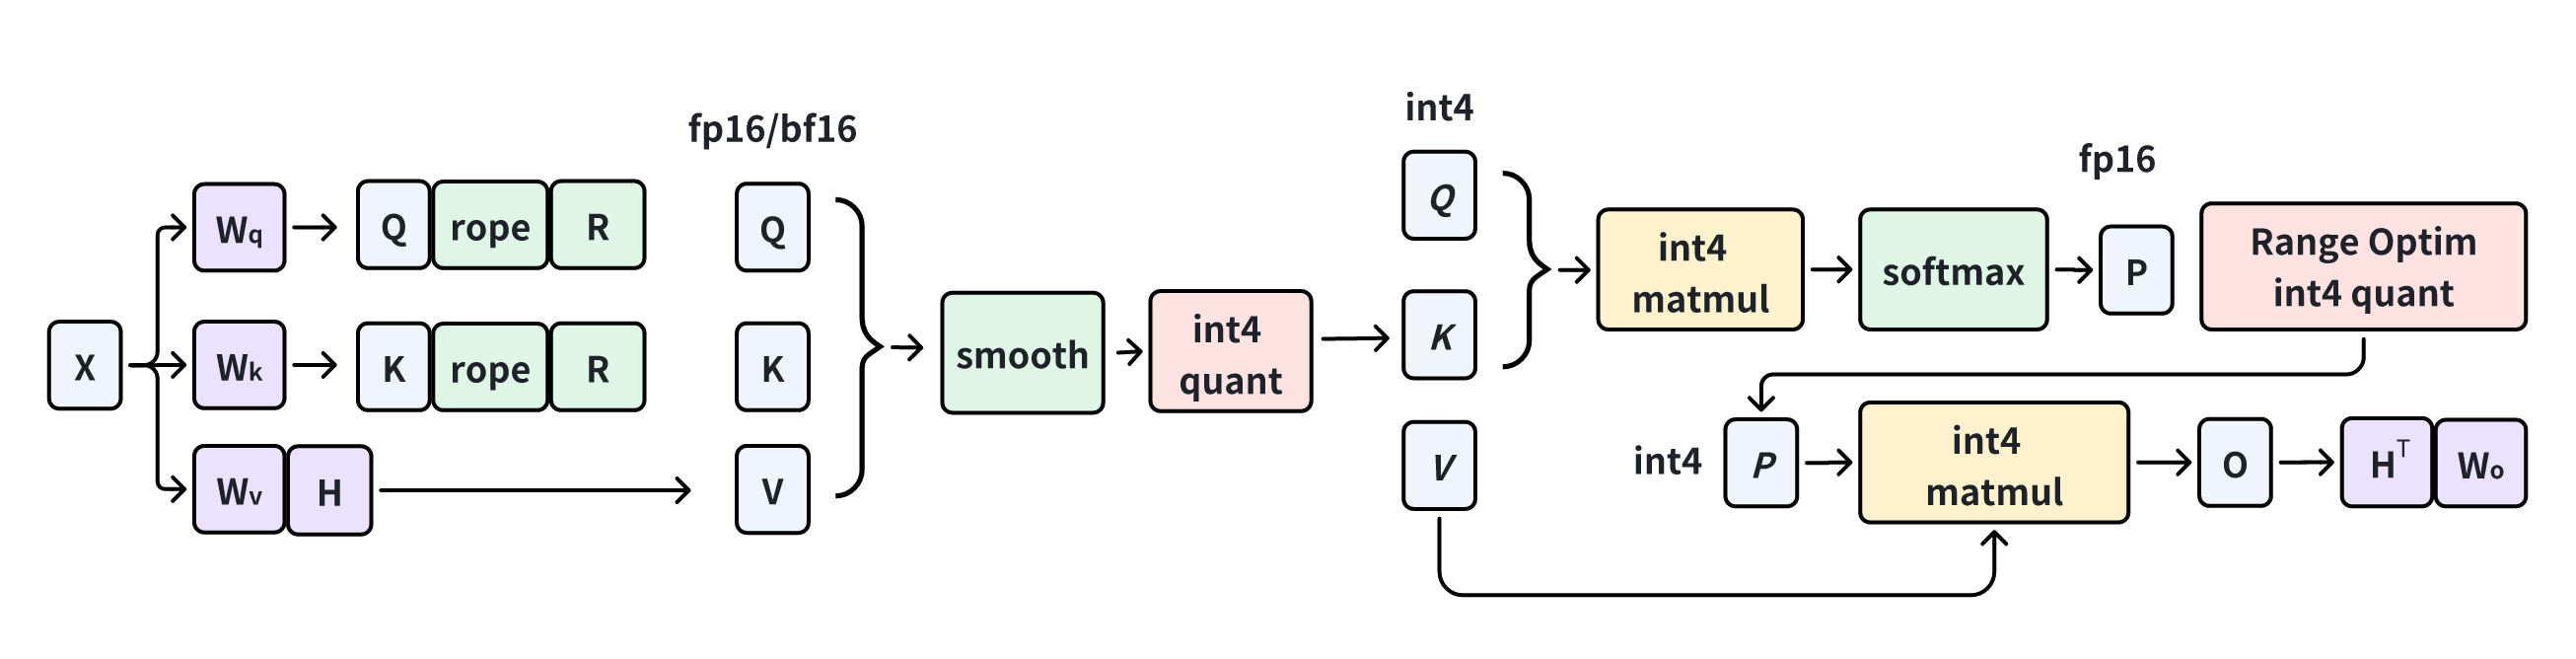
\includegraphics[width=0.92\linewidth]{rotateattention}
    \end{center}
    \small Overall pipeline: RoPE-aware rotation, range-optimized $\mathbf{P}$ quantization, and Hadamard $\mathbf{V}$ transform.
}

%%%%%%%%%%%%%%%%%%%%%%%%%%%%%%%%%%%%%%%%%%%%%%%%%%%%%%%%%%%%%%%%%%%%%%%%%%%%%%
\headerbox{\bf\color{blue} Method: RoPE-aware Rotation + Range-optimized $\mathbf{P}$}{name=method,column=2,row=0,span=3}{
    \begin{minipage}[t]{0.60\linewidth}
        \textbf{\color{blue}(1) RoPE-aware Rotation.} Block-diagonal orthogonal $\mathbf{R}=\mathrm{diag}(\{\mathbf{R}_i\})$, $\mathbf{R}_i\in\mathrm{O}(2)$.
        \begin{itemize}\compresslist
            \item \textbf{Interleaved:} $\mathrm{RoPE}(\mathbf{Q})\mathbf{R}=\mathbf{Q}(\mathbf{M}\mathbf{R})$ pre-fused (zero cost).
            \item \textbf{Half:} couples $d^j_i$ with $d^j_{i+D_j/2}$ within segment $j\in\{f,h,w\}$.
        \end{itemize}
        \textbf{\color{blue}(2) Range-optimized $\mathbf{P}$:} $\tilde{\mathbf{P}}=\lfloor \mathbf{P}/\max(\mathbf{P})\times15\rceil-8 \in (-8,7]$ (full 16 levels).\\[0.3em]
        \textbf{\color{blue}(3) Hadamard $\mathbf{V}$:} merge $\widetilde{\mathbf{W}}_v=\mathbf{W}_v\mathbf{H}$, $\widetilde{\mathbf{W}}_o=\mathbf{H}^\top\mathbf{W}_o$ offline.
    \end{minipage}\hfill
    \begin{minipage}[t]{0.37\linewidth}
        \centering
        \raisebox{-\height}{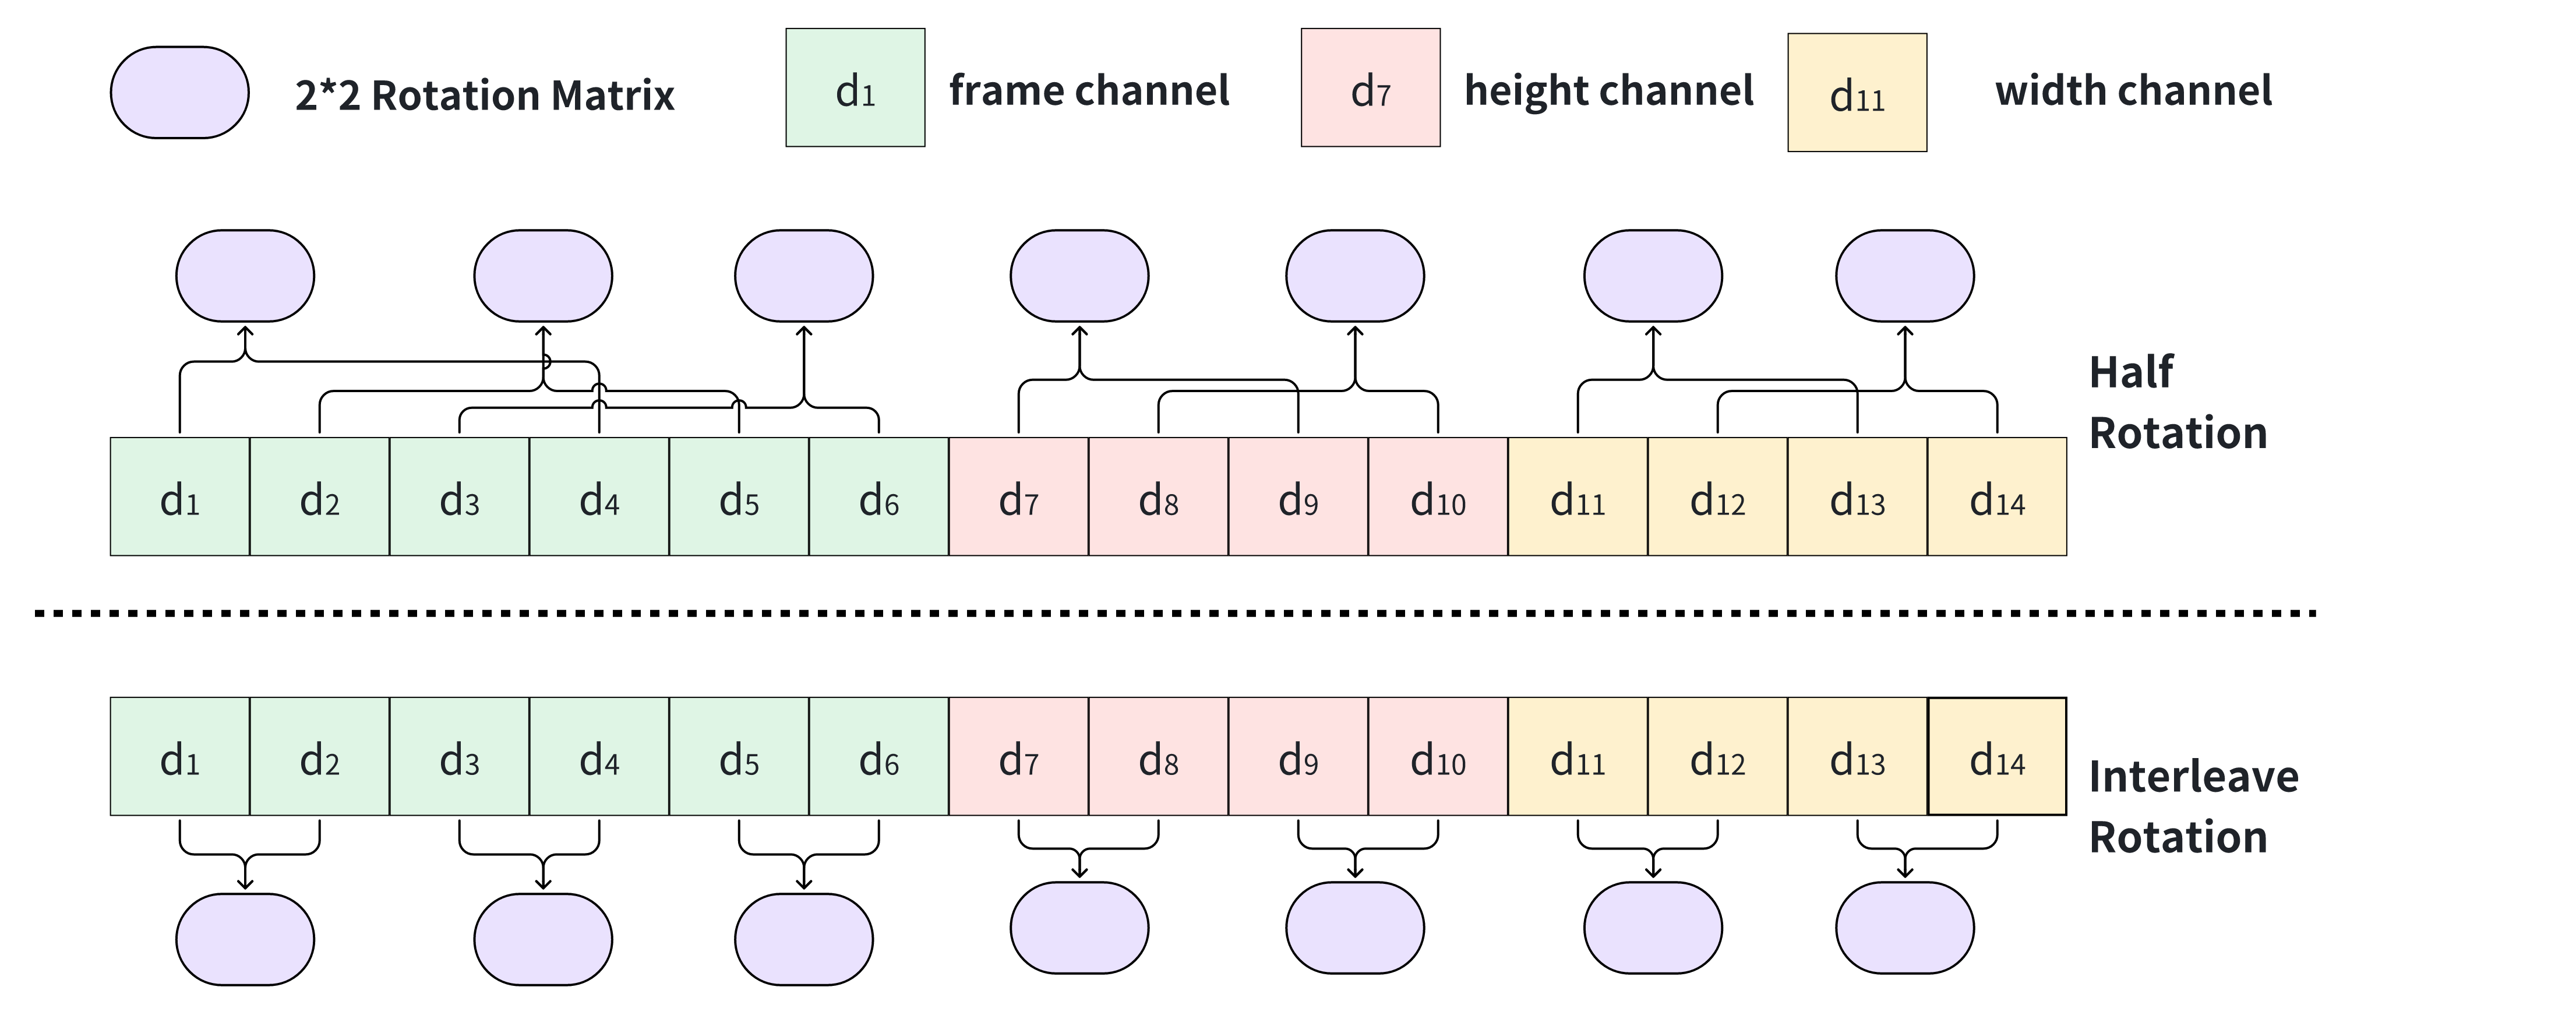
\includegraphics[width=\linewidth]{rotation}}
    \end{minipage}
}

\headerbox{\bf\color{blue} Outlier Analysis: What 3D RoPE Does to $\mathbf{Q}$/$\mathbf{K}$}{name=findings,column=0,below=problem,span=2}{
    \textbf{\color{blue}Metric:} $\Psi(\mathbf{X})=\max_i\big|\mathbf{X}_{i,:}-\mathbb{E}[\mathbf{X}]\big|$ (channel-level incoherence); 3D RoPE partitions $D=D_f+D_h+D_w$.
    \begin{itemize}\compresslist
        \item \textbf{Segmental incoherence:} outliers split into frame/height/width segments; one half of each segment dominates.
        \item \textbf{Cross-matrix symmetry:} $\mathbf{Q}$ and $\mathbf{K}$ share nearly identical incoherence.
    \end{itemize}

    \begin{center}
    \begin{minipage}[t]{0.42\linewidth}
        \centering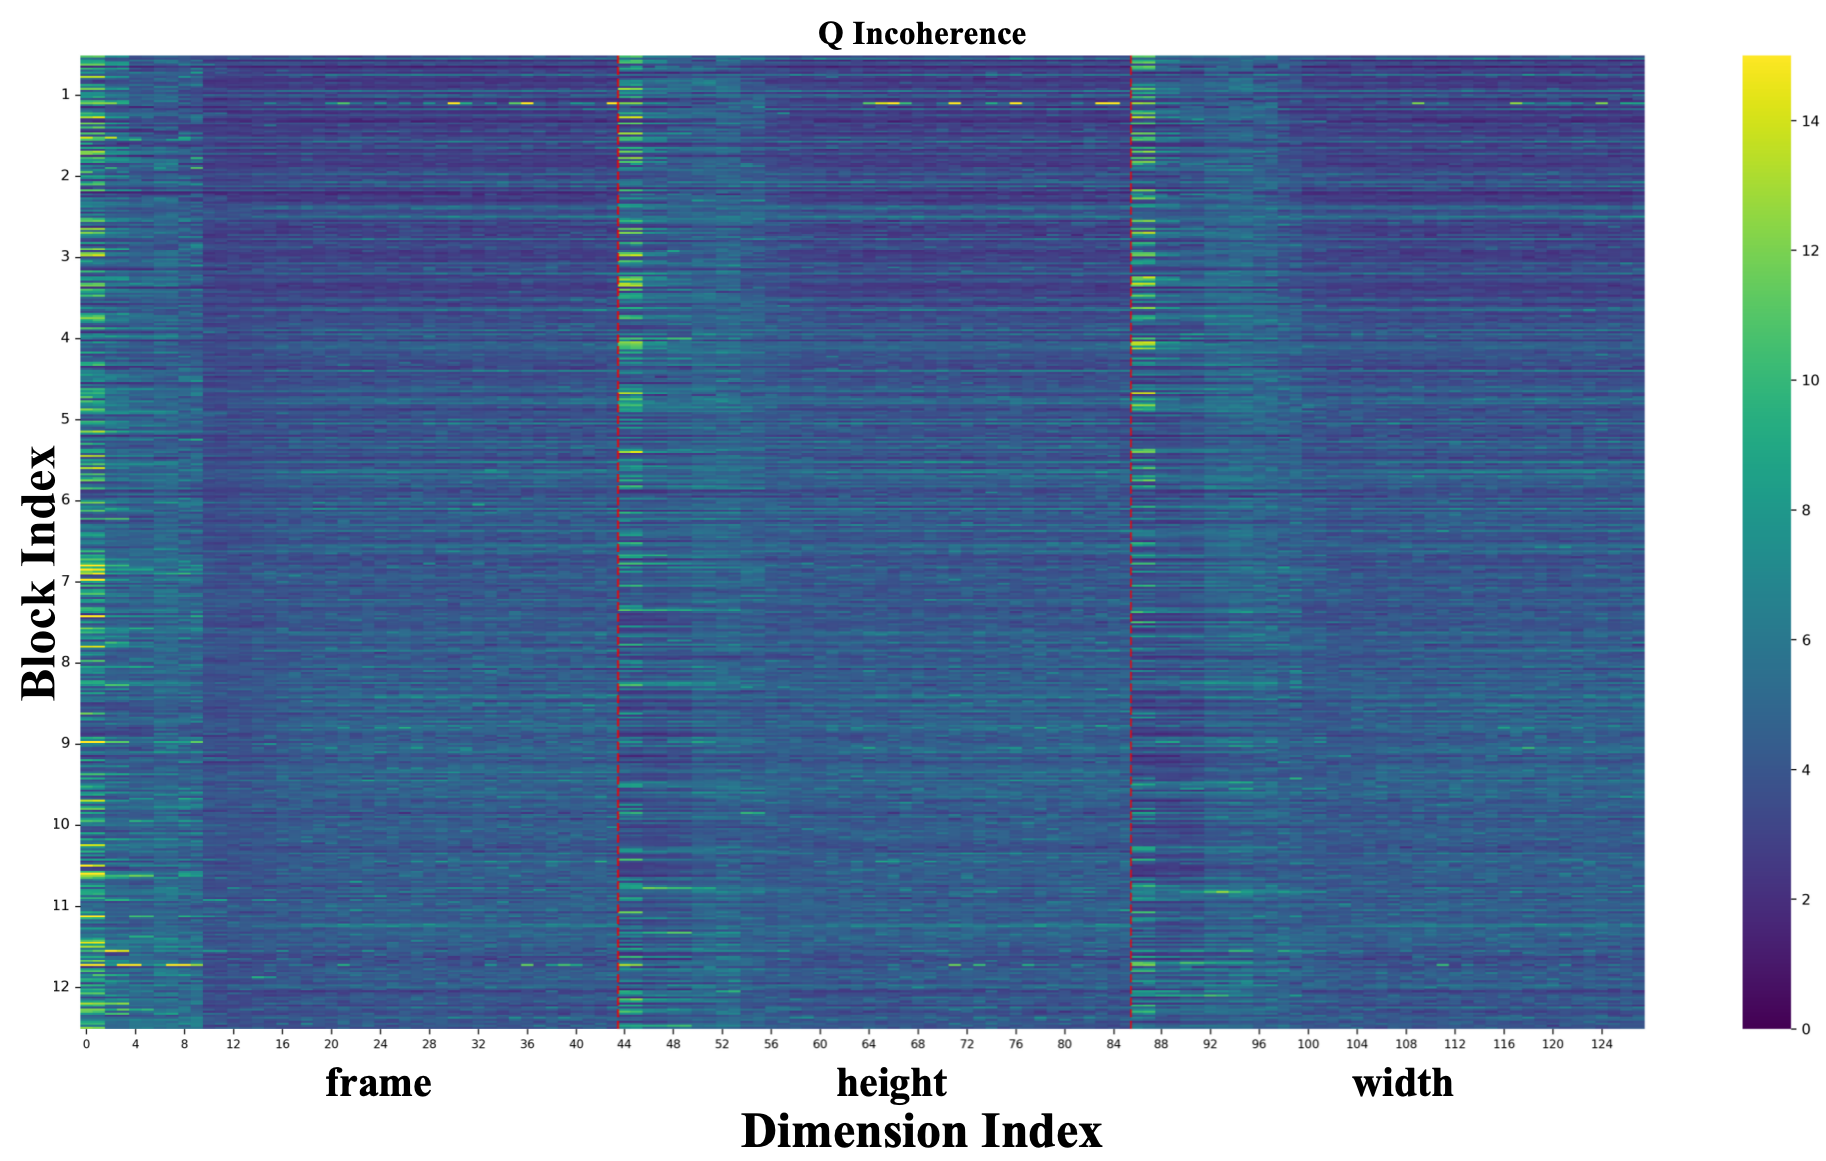
\includegraphics[width=\linewidth]{q1}\\[-0.2em]
        {\small $\mathbf{Q}$ (Wan2.2)}
    \end{minipage}\hfill
    \begin{minipage}[t]{0.42\linewidth}
        \centering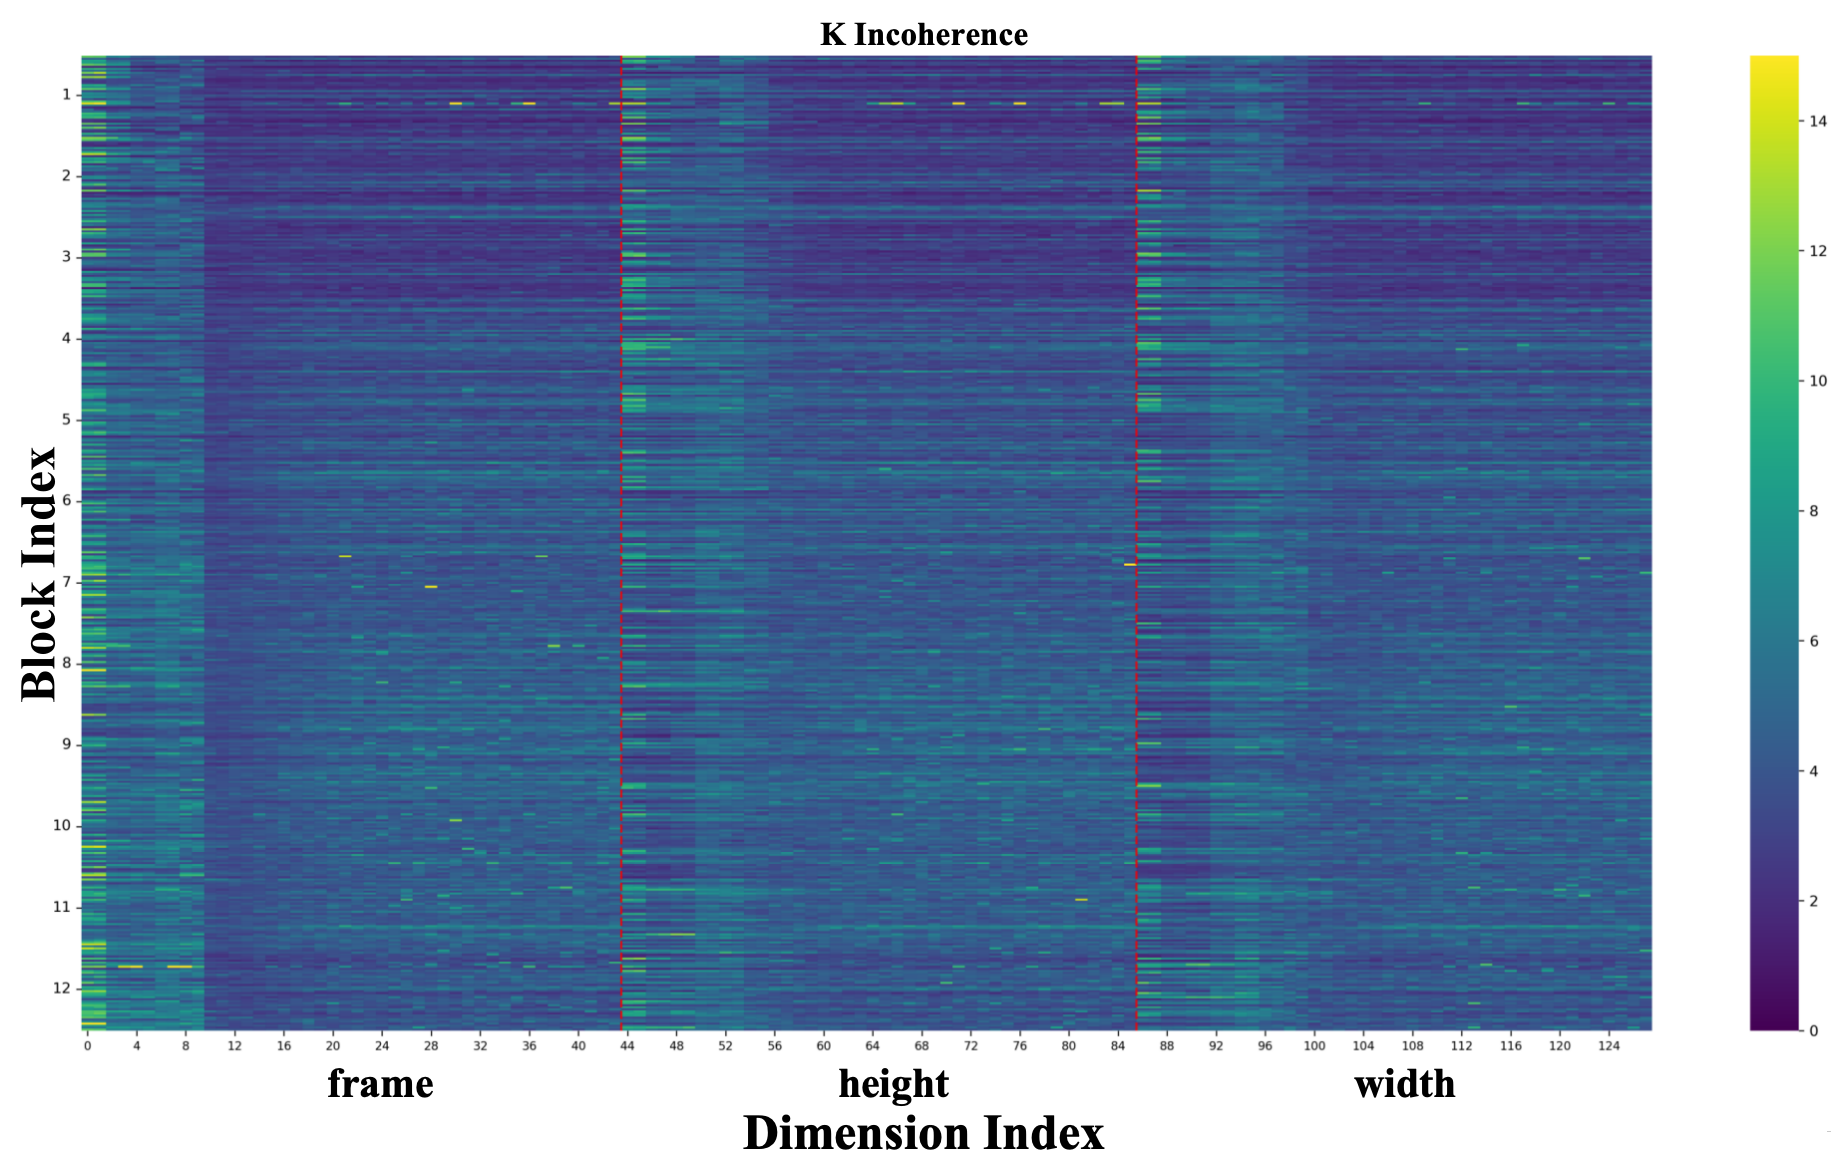
\includegraphics[width=\linewidth]{k1}\\[-0.2em]
        {\small $\mathbf{K}$ (Wan2.2)}
    \end{minipage}
    \end{center}

    \textbf{\color{blue}Take-away:} structured, symmetric patterns make \emph{orthogonal, RoPE-compatible} rotations the right tool.
}

%%%%%%%%%%%%%%%%%%%%%%%%%%%%%%%%%%%%%%%%%%%%%%%%%%%%%%%%%%%%%%%%%%%%%%%%%%%%%%
\headerbox{\bf\color{blue} Qualitative Results (Generated Video Frames)}{name=results,column=2,below=method,span=3}{
    \textbf{\color{blue}Wan2.2 T2V (top) and Wan2.2 I2V (bottom).} Our rotations with range-optimized $\mathbf{P}$ keep generated frames close to FP16 and clearly improve structure and temporal consistency over SageAttention.
    \begin{center}
    {\scriptsize
    \setlength{\tabcolsep}{1.5pt}
    \begin{tabular}{cccccc}
        FP16 & Full & Half & Interleave & W/O Rot & SageAttn \\
        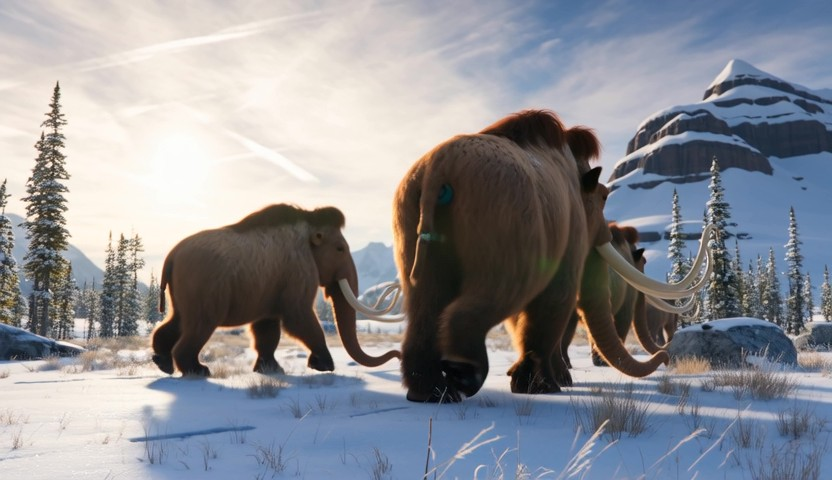
\includegraphics[width=0.16\linewidth]{t2v_fp} &
        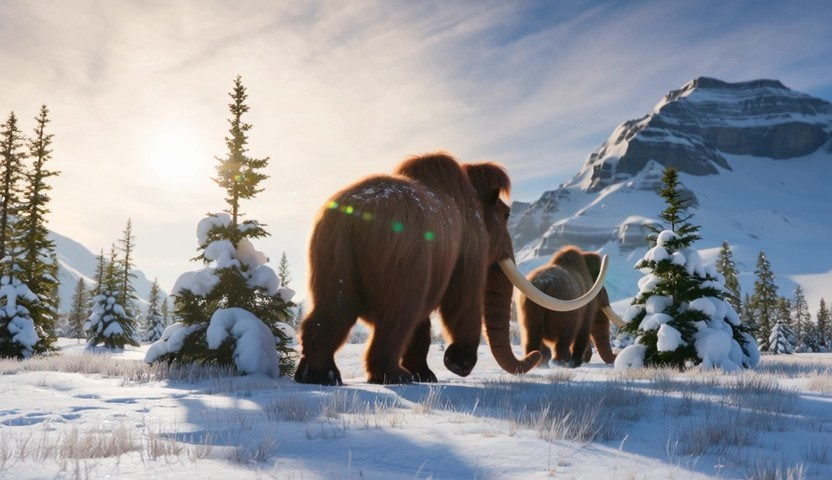
\includegraphics[width=0.16\linewidth]{t2v_full} &
        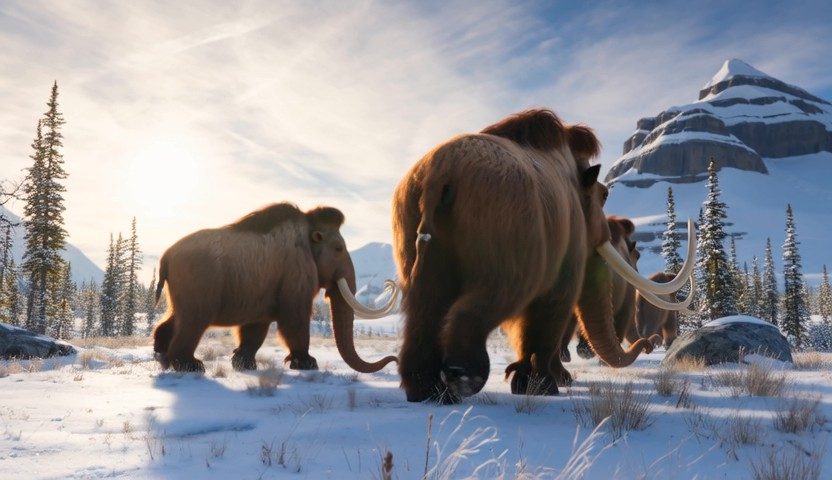
\includegraphics[width=0.16\linewidth]{t2v_half} &
        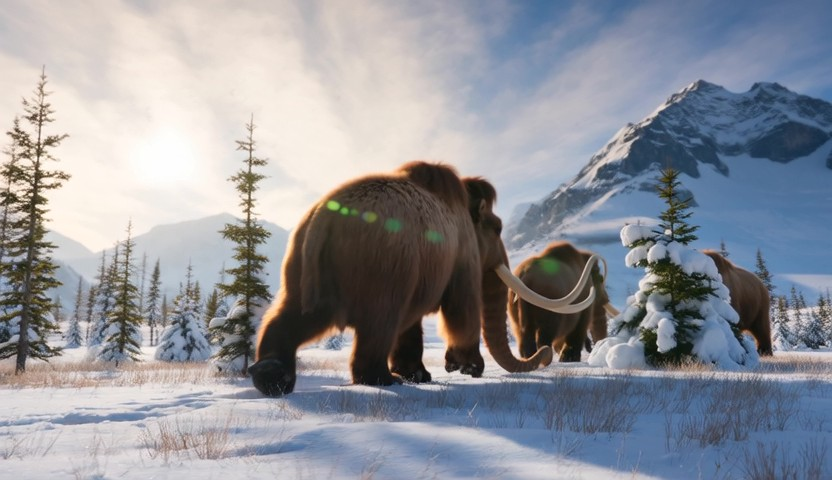
\includegraphics[width=0.16\linewidth]{t2v_inter} &
        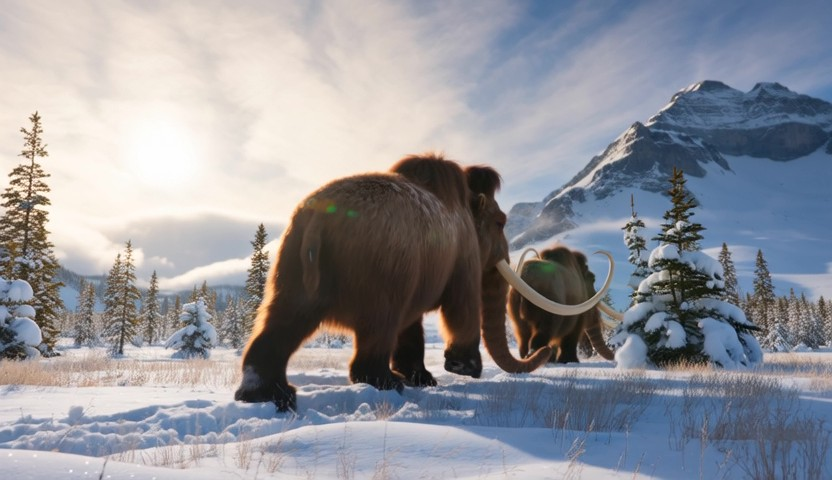
\includegraphics[width=0.16\linewidth]{t2v_wo_h} &
        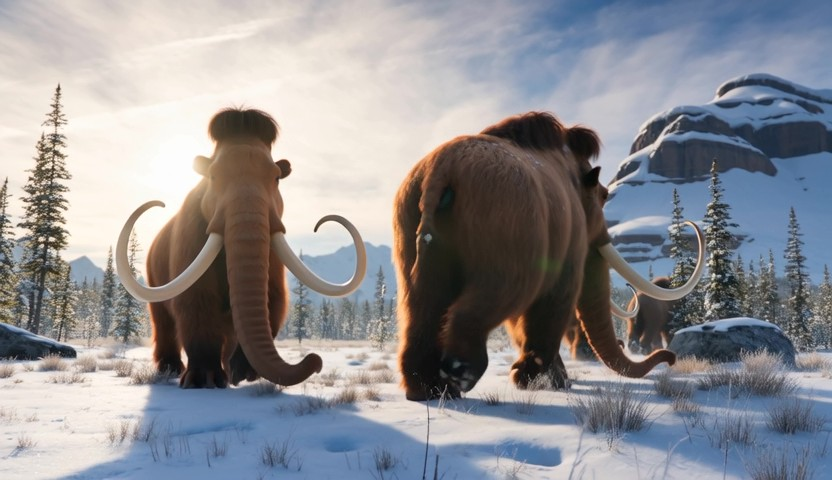
\includegraphics[width=0.16\linewidth]{t2v_sageattn} \\
        FP16 & Full & Half & Interleave & W/O Rot & SageAttn \\
        
\includegraphics[width=0.16\linewidth]{i2v_fp} &
        
\includegraphics[width=0.16\linewidth]{i2v_full} &
        
\includegraphics[width=0.16\linewidth]{i2v_half} &
        
\includegraphics[width=0.16\linewidth]{i2v_inter} &
        
\includegraphics[width=0.16\linewidth]{i2v_wo_h} &
        
\includegraphics[width=0.16\linewidth]{i2v_sageattn} \\
    \end{tabular}
    }
    \end{center}
}

%%%%%%%%%%%%%%%%%%%%%%%%%%%%%%%%%%%%%%%%%%%%%%%%%%%%%%%%%%%%%%%%%%%%%%%%%%%%%%
\headerbox{\bf\color{blue} Learned Rotation Must Be Orthogonal}{name=ortho,column=2,below=results,span=3}{
    \textbf{Learned rotations $\in \mathrm{O}(2)$} (orthogonal constraint).\\
    Limited rotation space: no clear quality gain, but no degradation.\\
    Without the constraint $\rightarrow$ degraded results.
    \begin{center}
    {\scriptsize
    \setlength{\tabcolsep}{4pt}
    \begin{tabular}{ccc}
        FP16 & Orthogonal & Unconstrained \\
        
\includegraphics[width=0.18\linewidth]{cat_fp16} &
        
\includegraphics[width=0.18\linewidth]{cat_train} &
        
\includegraphics[width=0.18\linewidth]{cat_train_nozj} \\
    \end{tabular}
    }
    \end{center}
}

\end{poster}
\end{document}
